% Decoder-model write-up (parallel structure to other/encoder.tex).
% Compile from LATEX_writeup/ with pdflatex (figures: ../Manova_Permanova_Results/<model>/*.png).
% If PNGs are missing, re-run the analysis cells in Jupyter_Codes or restore per-model PNGs.

\documentclass[11pt]{article}

\usepackage[margin=1in]{geometry}
\usepackage{booktabs}
\usepackage{array}
\usepackage{graphicx}
\usepackage{float}
\usepackage{subcaption}
\usepackage{amsmath}
\usepackage{amssymb}
\usepackage{hyperref}
\usepackage{caption}
\usepackage{xcolor}
\usepackage{setspace}
\usepackage{enumitem}

\captionsetup{font=small}
\setstretch{1.08}

\hypersetup{colorlinks=true, linkcolor=blue, urlcolor=blue, citecolor=blue}

\title{Decoder-Based (Causal) Language Models for Chunk-Conditioned\\
Question--Answer Generation: Experimental and Multivariate Statistical Evaluation}
\author{[Your Name]\\Michigan Technological University}
\date{}

\begin{document}

\maketitle

\begin{abstract}
This report documents the decoder-model track of our lab's document-processing pipeline for language-model customization. Where an encoder-based relevance classifier (see parallel lab write-up) filters chunks before downstream use, the present study evaluates \emph{causal}, instruction-tuned decoder models that generate question--answer pairs conditioned on each retained text chunk. Four open models are exercised under a factorial-style grid crossing chunking indices $\{128,256,512,1024\}$ with multiple maximum new-token budgets for generation. Aggregated outputs are scored with ROUGE (four variants), BERTScore (precision, recall, F1), and a semantic textual similarity (STS) signal derived from sentence embeddings.

For each model, the analysis pipeline includes exploratory visualization, correlation structure and variance inflation factors (VIF), diagnostic checks for multivariate normality (Henze--Zirkler), homogeneity of covariance (Box's~M), and multivariate outlier screening, followed by multivariate analysis of variance (MANOVA; Type~III) and permutational MANOVA (PERMANOVA; 999 permutations) on z-standardized metrics. Principal component analysis (PCA) illustrates separation of chunk-size groups in reduced space. Omnibus PERMANOVA indicates a statistically significant multivariate effect of chunk size for every model ($p=0.001$ in each saved summary), with pseudo-$F$ values ranking Qwen2.5-7B-Instruct highest, then Mistral-7B-Instruct-v0.3, Gemma (7B), and Phi-4-mini-instruct. Smaller chunk indices consistently align with higher automatic scores. Classical MANOVA assumptions are often violated (notably covariance heterogeneity and, for three models, multivariate normality), so PERMANOVA and descriptive multivariate views are treated as primary for inference. Artifacts are stored under \texttt{Jupyter\_Codes/}, \texttt{Codes\_Outputs/}, and \texttt{Manova\_Permanova\_Results/}.
\end{abstract}

\tableofcontents
\newpage

\section{Introduction}

Long-form documents in our workflow are first segmented into chunks. Encoder models address which chunks are semantically relevant; decoder models then consume those chunks (or, in the experiments reported here, chunks at controlled widths) to produce training-style question--answer data. Poor chunk sizing can dilute local context or overload the model, so understanding how chunk size interacts with decoder choice is central to pipeline design.

This study focuses \emph{exclusively} on the decoder stage: conditional generation of QA pairs and multivariate evaluation of generation quality under chunk-size manipulations. It is designed to parallel, not duplicate, the encoder-track report prepared separately.

\section{Task definition}

The decoder receives a single text chunk (and a fixed prompting template) and generates one or more question--answer pairs. Reference answers implied by the chunk text are used together with model outputs in standard automatic metrics. The task emulates retrieval-augmented generation in which the retriever supplies one chunk per query, so conclusions apply to ``single-chunk context'' settings rather than full-document prompts.

\section{Data, chunking, and run artifacts}

\subsection{Source material and chunking}

Experiments use chunked passages derived from PDF text prepared in the lab's segmentation workflow (\texttt{Generate\_Paragraphs/} notebook and JSON under \texttt{Generate\_Paragraphs/Results/}). Chunk stores are keyed by source PDF path; nominal chunking levels $128$, $256$, $512$, and $1024$ select among files such as \texttt{extracted\_chunks\_<size>\_overlap.json}. Each experimental cell corresponds to a combination of chunk level and a chosen maximum number of new tokens allocated to decoding.

\subsection{Stored outputs}

For each configuration, generations are logged as JSON files (e.g.\ \texttt{generation\_log\_<chunk>\_Token\_<maxtok>\_Q1.json}) mapping source paths to chunk text and \texttt{qa\_pairs}. Run manifests such as \texttt{qa\_run\_tracker\_detailed.csv} record success and failure counts per cell, supporting auditability across lab machines and run IDs (\texttt{NEW\_RUNS\_LMForge\_RUN01\_Lab\_Machine}, \texttt{RUN02}, \texttt{RUN04}, etc.).

\section{Model pool and experimental design}

\subsection{Decoder model pool}

Table~\ref{tab:decoder-pool} lists the four causal instruction-tuned models evaluated. Each has a dedicated Jupyter notebook under \texttt{Jupyter\_Codes/} with the same overall structure (load, generate, score, analyze).

\begin{table}[H]
\centering
\caption{Decoder model pool (Hugging Face identifiers as in lab notebooks)}
\label{tab:decoder-pool}
\begin{tabular}{ll}
\toprule
Display name & \texttt{model\_name} in notebook \\
\midrule
Gemma 7B & \texttt{google/gemma-7b} \\
Mistral 7B Instruct v0.3 & \texttt{mistralai/Mistral-7B-Instruct-v0.3} \\
Phi-4-mini-instruct & \texttt{microsoft/Phi-4-mini-instruct} \\
Qwen2.5-7B-Instruct & \texttt{Qwen/Qwen2.5-7B-Instruct} \\
\bottomrule
\end{tabular}
\end{table}

\noindent Aggregated results folders use the labels \texttt{gemma-7b-spark}, \texttt{Mistral-7B-Instruct-v0.3}, \texttt{Phi-4-mini-instruct}, and \texttt{Qwen2.5-7B-Instruct} under \texttt{Manova\_Permanova\_Results/}.

\subsection{Factors and design size}

Chunk size is the primary grouping factor for omnibus multivariate tests, with four levels $\{128,256,512,1024\}$. Maximum new tokens during decoding takes multiple levels (e.g.\ $128,256,512,1024,2048$), as reflected in output filenames and run trackers, yielding a grid of experimental cells. For the multivariate summaries exported to \texttt{statistical\_summary.txt}, the design has sample size $N=20$ observations and four chunk-size groups (five cells per chunk size in the crossed grid), with PERMANOVA based on $999$ permutations.

\subsection{Inference configuration}

Table~\ref{tab:decoder-hyper} summarizes shared implementation choices recorded in the notebooks (not exhaustive of every path variant).

\begin{table}[H]
\centering
\caption{Decoder inference settings (typical lab configuration)}
\label{tab:decoder-hyper}
\begin{tabular}{ll}
\toprule
Setting & Value \\
\midrule
Model class & \texttt{AutoModelForCausalLM} \\
Precision & \texttt{float16} on CUDA \\
Device & \texttt{device\_map="cuda"} where available \\
Batch size & Configurable (e.g.\ 10); set per run in notebook \\
\texttt{transformers} note & Notebook references 4.53.2 compatibility \\
Caching & \texttt{HF\_HOME} / hub cache on lab drive \\
\bottomrule
\end{tabular}
\end{table}

\section{Evaluation metrics}

Each analysis cell contributes a vector of eight dependent variables (means over items in that cell):
\begin{itemize}[noitemsep]
    \item ROUGE-1, ROUGE-2, ROUGE-L, ROUGE-Lsum;
    \item BERTScore precision, recall, and F1;
    \item STS score (embedding-based similarity).
\end{itemize}

ROUGE and BERTScore capture n-gram and token-level overlap with references; STS summarizes semantic proximity. Together they support a multivariate profile of quality, at the cost of substantial correlation among components (especially among ROUGE variants).

\section{Statistical validation}

\subsection{Exploratory and association structure}

Line plots and boxplots relate chunk size and max-new-token settings to BERTScore F1. Correlation heatmaps and VIF quantify redundancy. Reported VIFs for ROUGE components are very large, flagging linear multicollinearity that complicates interpretation of individual MANOVA coefficients.

\subsection{MANOVA assumptions}

\textbf{Multivariate normality} is assessed with the Henze--Zirkler test. In the archived summaries, normality is rejected for Gemma, Mistral, and Phi (very small $p$-values), while Qwen2.5 does not reject at $\alpha=0.05$ ($p\approx 0.09$).

\textbf{Homogeneity of covariance} is assessed with Box's~M; the saved output rejects equal covariances across chunk-size groups for all models, with $\chi^2$ reported as infinite in the log (numerical overflow under severe heterogeneity).

\textbf{Outliers} are flagged via Mahalanobis distance; approximately $25\%$ of the $N=20$ observations exceed the threshold at $p<0.001$ in each model's \texttt{outlier\_summary.csv}.

\subsection{MANOVA (Type III)}

Type~III MANOVA tables (Wilks' $\Lambda$, Pillai, Hotelling--Lawley, Roy) are computed for completeness. Because covariance homogeneity and outlier rates are problematic, these results are \emph{not} treated as the primary confirmatory basis.

\subsection{PERMANOVA}

PERMANOVA tests whether chunk-size groups differ on the \emph{joint} metric vector using permutations of Euclidean distances among z-scored outcomes. The omnibus pseudo-$F$ and permutation $p$-value are the main inferential summaries. Pairwise PERMANOVA contrasts adjacent and extreme chunk sizes; $p$-values are permutation-based and, with $B=999$, floor at $0.001$ when no permuted statistic exceeds the observed value.

\subsection{PCA}

PCA projects the dependent variables into two dimensions for visualization and supports auxiliary MANOVA on the first components where recorded in \texttt{statistical\_summary.txt}.

\section{Results}

\subsection{Mean outcomes by chunk size}

Tables~\ref{tab:means-gemma}--\ref{tab:means-qwen} report group means from each model's \texttt{group\_means.csv}. In every case, ROUGE and BERTScore F1 decrease as chunk size increases from 128 to 1024, consistent with the hypothesis that smaller local contexts yield more extractive, metric-friendly QA behavior under this protocol. Phi shows a non-monotone pattern on some ROUGE entries at 256 versus 128, but the 1024 condition remains clearly weakest overall.

\begin{table}[H]
\centering
\caption{Gemma (\texttt{gemma-7b-spark}): mean metrics by chunk size}
\label{tab:means-gemma}
\small
\begin{tabular}{rcccccccc}
\toprule
Chunk & R1 & R2 & RL & RLsum & BERT-P & BERT-R & BERT-F1 & STS \\
\midrule
128 & 0.375 & 0.270 & 0.317 & 0.357 & 0.730 & 0.513 & 0.593 & 0.608 \\
256 & 0.276 & 0.194 & 0.228 & 0.267 & 0.724 & 0.462 & 0.555 & 0.566 \\
512 & 0.200 & 0.145 & 0.170 & 0.196 & 0.727 & 0.445 & 0.547 & 0.557 \\
1024 & 0.108 & 0.072 & 0.089 & 0.106 & 0.652 & 0.412 & 0.500 & 0.480 \\
\bottomrule
\end{tabular}
\end{table}

\begin{table}[H]
\centering
\caption{Mistral-7B-Instruct-v0.3: mean metrics by chunk size}
\label{tab:means-mistral}
\small
\begin{tabular}{rcccccccc}
\toprule
Chunk & R1 & R2 & RL & RLsum & BERT-P & BERT-R & BERT-F1 & STS \\
\midrule
128 & 0.449 & 0.329 & 0.366 & 0.419 & 0.775 & 0.573 & 0.652 & 0.709 \\
256 & 0.309 & 0.230 & 0.254 & 0.295 & 0.775 & 0.500 & 0.603 & 0.654 \\
512 & 0.180 & 0.132 & 0.147 & 0.173 & 0.745 & 0.440 & 0.550 & 0.562 \\
1024 & 0.106 & 0.080 & 0.088 & 0.103 & 0.683 & 0.432 & 0.526 & 0.530 \\
\bottomrule
\end{tabular}
\end{table}

\begin{table}[H]
\centering
\caption{Phi-4-mini-instruct: mean metrics by chunk size}
\label{tab:means-phi}
\small
\begin{tabular}{rcccccccc}
\toprule
Chunk & R1 & R2 & RL & RLsum & BERT-P & BERT-R & BERT-F1 & STS \\
\midrule
128 & 0.404 & 0.215 & 0.267 & 0.357 & 0.651 & 0.591 & 0.610 & 0.723 \\
256 & 0.429 & 0.229 & 0.266 & 0.387 & 0.704 & 0.565 & 0.622 & 0.732 \\
512 & 0.318 & 0.163 & 0.191 & 0.295 & 0.698 & 0.507 & 0.582 & 0.605 \\
1024 & 0.164 & 0.073 & 0.096 & 0.154 & 0.596 & 0.440 & 0.502 & 0.495 \\
\bottomrule
\end{tabular}
\end{table}

\begin{table}[H]
\centering
\caption{Qwen2.5-7B-Instruct: mean metrics by chunk size}
\label{tab:means-qwen}
\small
\begin{tabular}{rcccccccc}
\toprule
Chunk & R1 & R2 & RL & RLsum & BERT-P & BERT-R & BERT-F1 & STS \\
\midrule
128 & 0.455 & 0.301 & 0.370 & 0.420 & 0.771 & 0.599 & 0.670 & 0.751 \\
256 & 0.351 & 0.236 & 0.279 & 0.329 & 0.771 & 0.539 & 0.631 & 0.714 \\
512 & 0.240 & 0.167 & 0.197 & 0.229 & 0.761 & 0.492 & 0.595 & 0.670 \\
1024 & 0.159 & 0.110 & 0.126 & 0.153 & 0.694 & 0.493 & 0.574 & 0.615 \\
\bottomrule
\end{tabular}
\end{table}

\subsection{Omnibus PERMANOVA and cross-model ranking}

Table~\ref{tab:permanova-omnibus} summarizes the chunk-size effect. All four models reject the null of equal multivariate location at the permutation threshold; the pseudo-$F$ magnitude orders models by how \emph{sharply} chunk sizes separate in metric space.

\begin{table}[H]
\centering
\caption{Omnibus PERMANOVA for chunk size ($N=20$, four groups, 999 permutations)}
\label{tab:permanova-omnibus}
\begin{tabular}{lcc}
\toprule
Model & Pseudo-$F$ & $p$ \\
\midrule
Qwen2.5-7B-Instruct & 220.85 & 0.001 \\
Mistral-7B-Instruct-v0.3 & 124.07 & 0.001 \\
gemma-7b-spark & 35.15 & 0.001 \\
Phi-4-mini-instruct & 13.63 & 0.001 \\
\bottomrule
\end{tabular}
\end{table}

\subsection{Pairwise PERMANOVA (illustrative)}

Table~\ref{tab:pairwise-mistral} and Table~\ref{tab:pairwise-phi} contrast two models with high versus low omnibus pseudo-$F$. For Mistral, even adjacent chunk sizes (e.g.\ 512 vs.\ 1024) yield small pairwise $p$-values. For Phi, the contrast 128 vs.\ 256 is not significant at $\alpha=0.05$ in the saved table ($p=0.462$), consistent with a flatter response to chunking.

\begin{table}[H]
\centering
\caption{Pairwise PERMANOVA: Mistral-7B-Instruct-v0.3 (\texttt{pairwise\_permanova.csv})}
\label{tab:pairwise-mistral}
\small
\begin{tabular}{rrrr}
\toprule
Group 1 & Group 2 & Pseudo-$F$ & $p$ \\
\midrule
128 & 256 & 55.44 & 0.012 \\
128 & 512 & 231.94 & 0.011 \\
128 & 1024 & 538.59 & 0.007 \\
256 & 512 & 35.04 & 0.011 \\
256 & 1024 & 102.31 & 0.011 \\
512 & 1024 & 14.47 & 0.007 \\
\bottomrule
\end{tabular}
\end{table}

\begin{table}[H]
\centering
\caption{Pairwise PERMANOVA: Phi-4-mini-instruct (\texttt{pairwise\_permanova.csv})}
\label{tab:pairwise-phi}
\small
\begin{tabular}{rrrr}
\toprule
Group 1 & Group 2 & Pseudo-$F$ & $p$ \\
\midrule
128 & 256 & 0.69 & 0.462 \\
128 & 512 & 4.27 & 0.041 \\
128 & 1024 & 37.05 & 0.010 \\
256 & 512 & 4.75 & 0.036 \\
256 & 1024 & 38.70 & 0.007 \\
512 & 1024 & 10.03 & 0.041 \\
\bottomrule
\end{tabular}
\end{table}

\section{Discussion}

Four substantive points mirror the style of conclusion in the encoder write-up, but for generation rather than classification.

First, \textbf{chunk size is a first-order lever} for decoder QA quality under automatic metrics: omnibus PERMANOVA is significant for every model, and mean tables show large drops between 128- and 1024-token chunks.

Second, \textbf{models differ in sensitivity}. Qwen2.5 and Mistral exhibit the largest pseudo-$F$ values, implying cleaner separation of chunk-size profiles; Phi is comparatively robust to moderate chunk-size changes, as seen in the non-significant 128 vs.\ 256 pairwise contrast. Gemma occupies an intermediate position. This argues against a single global chunk policy without reference to the chosen decoder.

Third, \textbf{classical MANOVA is a poor primary tool} here: heterogeneous covariances, abundant multivariate outliers, and multicollinearity among metrics undermine parametric multivariate inference. PERMANOVA on standardized distances aligns better with the data geometry while still testing a meaningful multivariate null.

Fourth, \textbf{integration with the encoder track}: smaller chunks may score better partly because they localize answerable content; the encoder filter and the decoder chunk size should be co-designed so that relevance and local coherence are jointly optimized.

\section{Conclusion}

This report presented the decoder-based experimental and statistical evaluation for chunk-conditioned question--answer generation. Four instruction-tuned causal LMs were tested under a controlled chunking and decoding grid, scored with eight correlated metrics, and analyzed with assumption-aware multivariate methods. Chunk size has a significant multivariate effect in every case; effect strength and pairwise patterns differ by architecture. Future work should enlarge $N$, add prompt variants, and validate automatic metrics against human judgments.

\section{Figures}

Figure~\ref{fig:bert-lines} shows BERTScore F1 versus experimental conditions for all four decoders. In each panel, performance tends to fall as chunk size increases, with additional structure from the max-new-token facet encoded in the plot.

\begin{figure}[H]
\centering
\begin{subfigure}{0.48\textwidth}
\centering

\includegraphics[width=\linewidth]{../Manova_Permanova_Results/gemma-7b-spark/lineplot_bert_f1.png}
\caption{Gemma (\texttt{gemma-7b-spark})}
\end{subfigure}\hfill
\begin{subfigure}{0.48\textwidth}
\centering
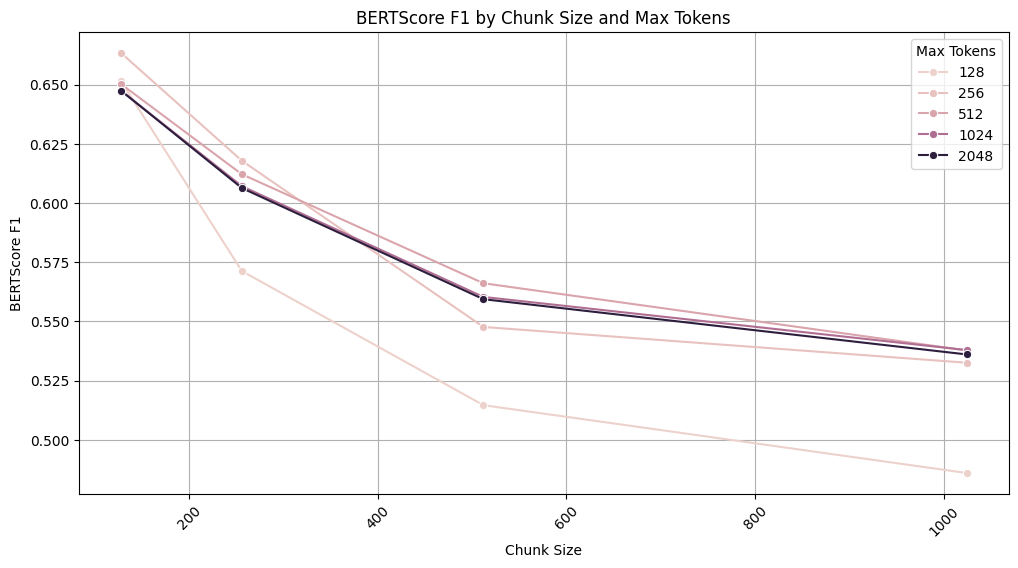
\includegraphics[width=\linewidth]{../Manova_Permanova_Results/Mistral-7B-Instruct-v0.3/lineplot_bert_f1.png}
\caption{Mistral-7B-Instruct-v0.3}
\end{subfigure}

\vspace{0.6em}

\begin{subfigure}{0.48\textwidth}
\centering

\includegraphics[width=\linewidth]{../Manova_Permanova_Results/Phi-4-mini-instruct/lineplot_bert_f1.png}
\caption{Phi-4-mini-instruct}
\end{subfigure}\hfill
\begin{subfigure}{0.48\textwidth}
\centering

\includegraphics[width=\linewidth]{../Manova_Permanova_Results/Qwen2.5-7B-Instruct/lineplot_bert_f1.png}
\caption{Qwen2.5-7B-Instruct}
\end{subfigure}
\caption{BERTScore F1 by chunk size and max new tokens (four decoder models).}
\label{fig:bert-lines}
\end{figure}

Figure~\ref{fig:bert-box} displays the distribution of BERTScore F1 across chunk sizes. Narrower boxes at small chunks and wider spread at large chunks indicate more stable generation when context is localized.

\begin{figure}[H]
\centering
\begin{subfigure}{0.48\textwidth}
\centering

\includegraphics[width=\linewidth]{../Manova_Permanova_Results/gemma-7b-spark/boxplot_bert_f1.png}
\caption{Gemma}
\end{subfigure}\hfill
\begin{subfigure}{0.48\textwidth}
\centering
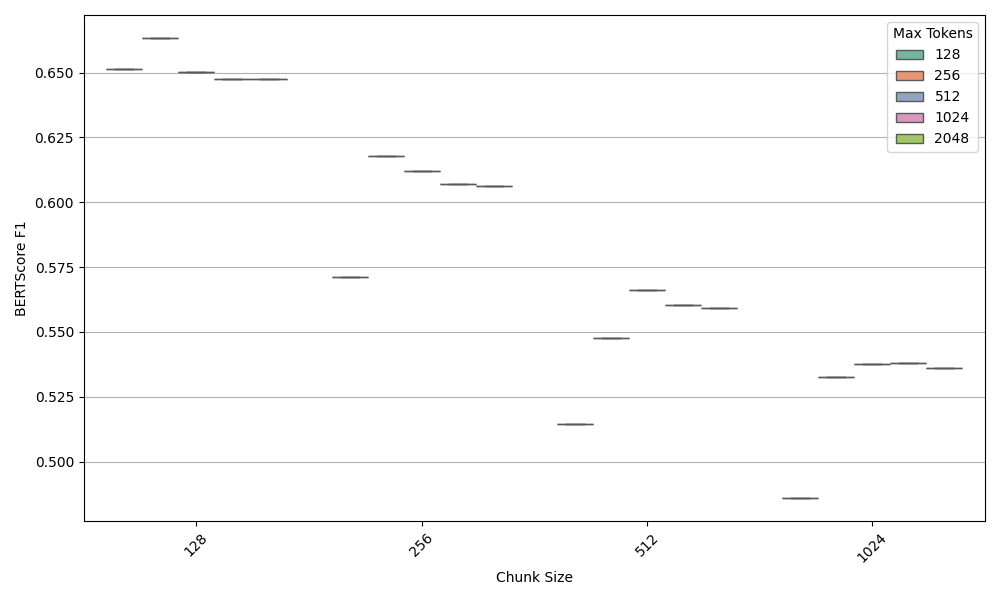
\includegraphics[width=\linewidth]{../Manova_Permanova_Results/Mistral-7B-Instruct-v0.3/boxplot_bert_f1.png}
\caption{Mistral}
\end{subfigure}

\vspace{0.6em}

\begin{subfigure}{0.48\textwidth}
\centering

\includegraphics[width=\linewidth]{../Manova_Permanova_Results/Phi-4-mini-instruct/boxplot_bert_f1.png}
\caption{Phi}
\end{subfigure}\hfill
\begin{subfigure}{0.48\textwidth}
\centering

\includegraphics[width=\linewidth]{../Manova_Permanova_Results/Qwen2.5-7B-Instruct/boxplot_bert_f1.png}
\caption{Qwen2.5}
\end{subfigure}
\caption{Boxplots of BERTScore F1 across chunk sizes.}
\label{fig:bert-box}
\end{figure}

Figure~\ref{fig:corr} highlights metric redundancy: ROUGE variants are almost perfectly correlated with each other in several panels, supporting reliance on multivariate distance-based tests rather than eight independent univariate narratives.

\begin{figure}[H]
\centering
\begin{subfigure}{0.48\textwidth}
\centering

\includegraphics[width=\linewidth]{../Manova_Permanova_Results/gemma-7b-spark/correlation_heatmap.png}
\caption{Gemma}
\end{subfigure}\hfill
\begin{subfigure}{0.48\textwidth}
\centering

\includegraphics[width=\linewidth]{../Manova_Permanova_Results/Mistral-7B-Instruct-v0.3/correlation_heatmap.png}
\caption{Mistral}
\end{subfigure}

\vspace{0.6em}

\begin{subfigure}{0.48\textwidth}
\centering

\includegraphics[width=\linewidth]{../Manova_Permanova_Results/Phi-4-mini-instruct/correlation_heatmap.png}
\caption{Phi}
\end{subfigure}\hfill
\begin{subfigure}{0.48\textwidth}
\centering

\includegraphics[width=\linewidth]{../Manova_Permanova_Results/Qwen2.5-7B-Instruct/correlation_heatmap.png}
\caption{Qwen2.5}
\end{subfigure}
\caption{Correlation heatmaps of evaluation metrics (multicollinearity visible across models).}
\label{fig:corr}
\end{figure}

Figure~\ref{fig:qq} supports the Henze--Zirkler conclusions: substantial curvature away from the reference line appears for Gemma, Mistral, and Phi, while Qwen2.5 is closer to the diagonal (consistent with the marginal normality result).

\begin{figure}[H]
\centering
\begin{subfigure}{0.48\textwidth}
\centering

\includegraphics[width=\linewidth]{../Manova_Permanova_Results/gemma-7b-spark/qq_plot_mahalanobis.png}
\caption{Gemma}
\end{subfigure}\hfill
\begin{subfigure}{0.48\textwidth}
\centering

\includegraphics[width=\linewidth]{../Manova_Permanova_Results/Mistral-7B-Instruct-v0.3/qq_plot_mahalanobis.png}
\caption{Mistral}
\end{subfigure}

\vspace{0.6em}

\begin{subfigure}{0.48\textwidth}
\centering

\includegraphics[width=\linewidth]{../Manova_Permanova_Results/Phi-4-mini-instruct/qq_plot_mahalanobis.png}
\caption{Phi}
\end{subfigure}\hfill
\begin{subfigure}{0.48\textwidth}
\centering

\includegraphics[width=\linewidth]{../Manova_Permanova_Results/Qwen2.5-7B-Instruct/qq_plot_mahalanobis.png}
\caption{Qwen2.5}
\end{subfigure}
\caption{Q--Q plots of Mahalanobis distances (multivariate normality diagnostic).}
\label{fig:qq}
\end{figure}

Figure~\ref{fig:pca} visualizes chunk-size separation in PCA space. Models with larger omnibus pseudo-$F$ tend to show tighter, more separated clusters by chunk size; Phi shows more overlap, matching its smaller pseudo-$F$.

\begin{figure}[H]
\centering
\begin{subfigure}{0.48\textwidth}
\centering

\includegraphics[width=\linewidth]{../Manova_Permanova_Results/gemma-7b-spark/pca_scatter.png}
\caption{Gemma}
\end{subfigure}\hfill
\begin{subfigure}{0.48\textwidth}
\centering

\includegraphics[width=\linewidth]{../Manova_Permanova_Results/Mistral-7B-Instruct-v0.3/pca_scatter.png}
\caption{Mistral}
\end{subfigure}

\vspace{0.6em}

\begin{subfigure}{0.48\textwidth}
\centering

\includegraphics[width=\linewidth]{../Manova_Permanova_Results/Phi-4-mini-instruct/pca_scatter.png}
\caption{Phi}
\end{subfigure}\hfill
\begin{subfigure}{0.48\textwidth}
\centering

\includegraphics[width=\linewidth]{../Manova_Permanova_Results/Qwen2.5-7B-Instruct/pca_scatter.png}
\caption{Qwen2.5}
\end{subfigure}
\caption{PCA scatter of dependent variables colored by chunk size.}
\label{fig:pca}
\end{figure}

\appendix

\section{Artifact index}

Per model directory under \texttt{Manova\_Permanova\_Results/<model>/} also contains \texttt{anova\_type3\_results.csv}, \texttt{mean\_differences.csv}, \texttt{pairwise\_ttests\_fdr.csv}, \texttt{vif\_multicollinearity.csv}, \texttt{outliers\_detected.csv}, \texttt{outlier\_summary.csv}, and \texttt{statistical\_summary.txt}.

\end{document}
